% !TeX program = pdflatex
\documentclass[11pt,a4paper]{article}
\usepackage[utf8]{inputenc}
\usepackage[T1]{fontenc}
\usepackage[turkish]{babel}
\usepackage{lmodern}
\usepackage{geometry}
\usepackage{graphicx}
\usepackage{float}
\usepackage[section]{placeins}
\usepackage{flafter}
\usepackage{caption}
\usepackage{subcaption}
\usepackage{booktabs}
\usepackage{siunitx}
\usepackage{hyperref}
\usepackage{longtable}
\usepackage{xcolor}
\usepackage{microtype}
\usepackage{etoolbox}

\geometry{margin=1.5cm}
\hypersetup{colorlinks=true,linkcolor=blue,citecolor=blue,urlcolor=blue}
\graphicspath{{../results/}}
% Görsel ölçekleme: varsayılan genişlik ve oranı koru
\setkeys{Gin}{width=0.9\linewidth, keepaspectratio}

% Yüzen nesneleri başlık altında tutmak için sıkı kurallar
\floatplacement{figure}{H}
\floatplacement{table}{H}
\captionsetup{font=small,labelfont=bf}
\preto\section{\FloatBarrier}
\preto\subsection{\FloatBarrier}
\AfterEndEnvironment{figure}{\FloatBarrier}
\AfterEndEnvironment{table}{\FloatBarrier}
\AfterEndEnvironment{longtable}{\FloatBarrier}

\title{NPM Ekosisteminde Yönlü Karmaşık Ağ Analizi}
\author{\textbf{Yusuf Talha ARABACI}}
\date{\today}

\begin{document}
\maketitle

\begin{abstract}
Bu çalışma, NPM ekosistemindeki popüler paketler arasındaki bağımlılık ilişkilerini yönlü bir karmaşık ağ (Dependent $\to$ Dependency) olarak modeller ve ağın yapısal risklerini merkeziyet ölçütleriyle nicel olarak inceler. Veri, her çalıştırmada API'lerden (öncelik ecosyste.ms; yedek olarak npm registry ve npms.io) çekilir. Ağ NetworkX ile kurulup in-degree, out-degree ve betweenness merkeziyetleri hesaplanır; büyük graflarda betweenness örnekleme ($k$) ile hızlandırılır. Çalışma, merkeziyetlere dayalı bileşik bir risk skoru ile kritik düğümlerin sıralanmasını ve risk odaklı sağlamlık (robustluk) analizini (kritik düğümlerin çıkarılması) sunar. Üretilen tüm çıktılar results/ dizinindedir.
\end{abstract}

\clearpage

\section{Giriş ve Amaç}
Modern yazılım tedarik zincirinde tek bir bağımlılıktaki hata veya kasıtlı bir saldırı, transitif bağımlılıklar üzerinden yüzlerce hatta binlerce projeye yayılabilir. NPM ekosistemi; büyük ölçek, hızlı sürüm döngüleri ve yoğun bağımlılık grafiği nedeniyle bu tür zincirleme risklere özellikle açıktır. Bu rapor, paket içeriğinden ziyade paketler arası ilişkinin topolojik yapısına odaklanır: Bir paketin ağ içindeki konumu ve bu konumun sistemik etkileri nicel olarak değerlendirilir.

Bu çalışmanın hedefi, NPM bağımlılıklarını yönlü bir ağ olarak modelleyip yapısal riski görünür kılmaktır. Bunun için:
\begin{itemize}
  \item Bağımlı $\to$ bağımlılık yönünde kurulan ağ üzerinde, omurga ve köprü niteliğindeki paketleri merkeziyet ölçütleriyle (in-degree, out-degree, betweenness) belirliyoruz.
  \item Bu ölçütlerden türetilen bileşik bir risk skoru ile paketleri karşılaştırılabilir biçimde sıralıyoruz.
  \item Kritik düğümlerin çıkarılmasına dayalı sağlamlık göstergeleriyle (zayıf bileşen sayısı, en büyük bileşen boyutu vb.) ağın kırılganlığını nicel olarak değerlendiriyoruz.
\end{itemize}
Bu yaklaşım, güvenlik değerlendirmesini yalnızca paket içi zafiyetlere indirgemek yerine, bağımlılık topolojisinden kaynaklanan yapısal riskin de hesaba katılmasını sağlar. Böylece bakımı yapılacak, yakından izlenecek veya kısıtlanacak paketler veri temelli biçimde önceliklendirilebilir.

\section{Kuramsal Çerçeve ve Tanımlar}
\textbf{Yönlü Ağ (DiGraph).} Düğümler paketleri, yönlü kenarlar ise ``bağımlı $\to$ bağımlılık'' ilişkisini temsil eder. Bir paketin başka bir paketi kullanması, bağımlı paketten bağımlılığa giden bir ok (out-edge) olarak modellenir.

\textbf{In-degree.} Bir düğüme gelen kenar sayısıdır; başka kaç paket o pakete bağımlıdır. Yüksek in-degree, yayılım potansiyelini ve omurga olma riskini işaret eder.

\textbf{Out-degree.} Bir düğümden çıkan kenar sayısıdır; paketin kaç bağımlılığı vardır. Yüksek out-degree, geniş bağımlılık yüzeyi ve tedarik riskine maruziyet anlamına gelir.

\textbf{Betweenness Merkeziyeti.} En kısa yollar üzerinde bir düğümün köprü (aracılık) rolünü ölçer. Ağın topolojik boğaz noktalarını belirler; saldırı/bozulma durumunda tek hata noktalarına işaret edebilir.

\textbf{Bileşik Risk Skoru.} Normalize edilmiş (min--max) in/out/betweenness ölçülerinin ağırlıklı toplamıdır:
\[\mathrm{risk}(n) = w_{in}\,\tilde d_{in}(n) + w_{out}\,\tilde d_{out}(n) + w_b\,\tilde b(n)\]
Burada $\tilde x = (x - x_{\min})/(x_{\max}-x_{\min})$ min--max normalizasyonudur (payda sıfırsa $\tilde x=0$). Ağırlıklar $w_{in}, w_{out}, w_b$, omurga duyarlılığı (in-degree), bağımlılık yüzeyi (out-degree) ve köprü rolü (betweenness) arasında vurguyu dengeler.

\textbf{Sağlamlık (Robustluk) ve Kaskad Etkisi.} Risk sıralamasına göre en kritik düğümler çıkarıldığında zayıf bağlanırlık bileşen sayısı, en büyük bileşen boyutu ve (mümkünse) ağ çapı ölçülür. Kaskad etkisi, bir düğümün ele geçirilmesinin transitif olarak etkileyebileceği paket sayısını ifade eder.

\section{Veri ve Yöntem}
\textbf{Kaynaklar.} Top~N paket listeleri ve bağımlılıklar öncelikle ecosyste.ms API’lerinden; yedek olarak npm registry ve npms.io üzerinden alınır. Varsayılan olarak dependencies alanı kullanılır; isteğe bağlı olarak peerDependencies dahil edilebilir.

\textbf{Ağın Kurulumu.} Bağımlı $\to$ bağımlılık yönüyle NetworkX’te DiGraph oluşturulur. Tüm düğümler için in/out-degree; büyük graflarda örneklemeli ($k$) betweenness hesaplanır. Görseller ve tablolar results/ altında üretilir.

\textbf{Risk Skoru.} Ölçüler min--max normalize edilip ağırlıklı toplanır. Ağırlıklar (örn. $w_{in}=0.5$, $w_{out}=0.2$, $w_b=0.3$), omurga duyarlılığı, bağımlılık yüzeyi ve köprü rolü arasında denge kuran bir çerçeve sağlar.

\textbf{Sağlamlık Analizi.} Risk skoruna göre en kritik $k\in\{1,3,5\}$ düğüm çıkarılır; zayıf bileşen sayısı, en büyük bileşen boyutu ve varsa ağ çapı raporlanır (robustness\_risk.json).

\section{Bulgular ve Yorum}
Bu bölümde, results/ dizininden seçilen görseller/tablolar sunulur ve her biri doğrudan altında yorumlanır.

\subsection{Ağın Genel Görünümü}
\begin{figure}[H]
  \centering
  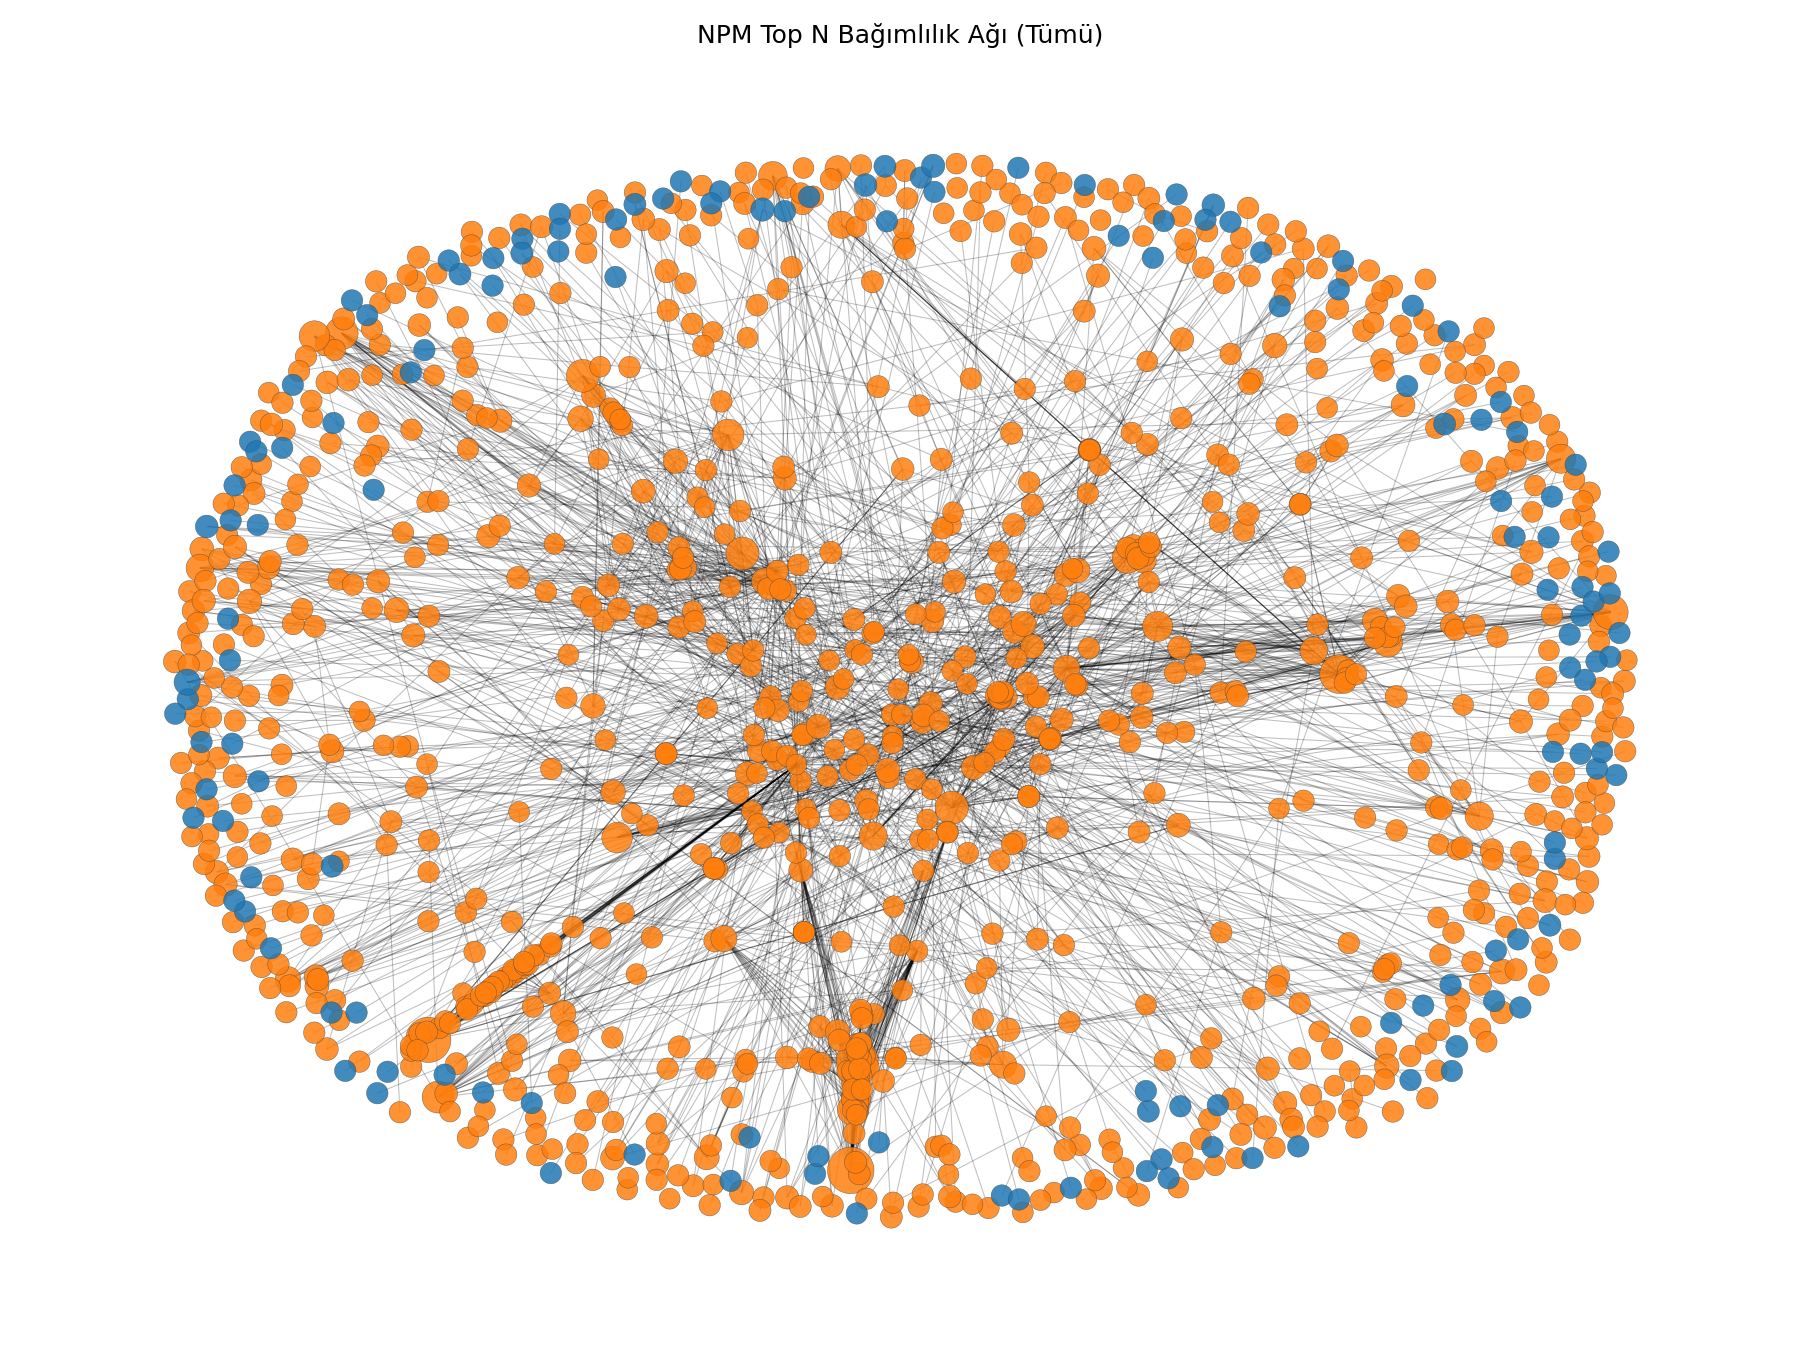
\includegraphics{network_full_topN.png}
  \caption{Top~N ve bağımlılıklarının oluşturduğu yönlü ağ. Düğüm boyutu in-degree ile, renkler Top~N (turuncu) ve diğerleri (mavi) olarak kodlanmıştır. Yüksek in-degree’li düğümler ekosistemin omurgasını oluşturur; bu düğümlerdeki sorunlar geniş yayılıma neden olabilir.}
\end{figure}

\noindent Bu görsel, merkezî kümelenmeleri ve omurga düğümleri ayırt etmeyi kolaylaştırır. Düğümler arası yüksek yoğunluklu bölgeler, paket ekosistemindeki tekrar eden birlikte-kullanım kalıplarına işaret eder.

\begin{figure}[H]
  \centering
  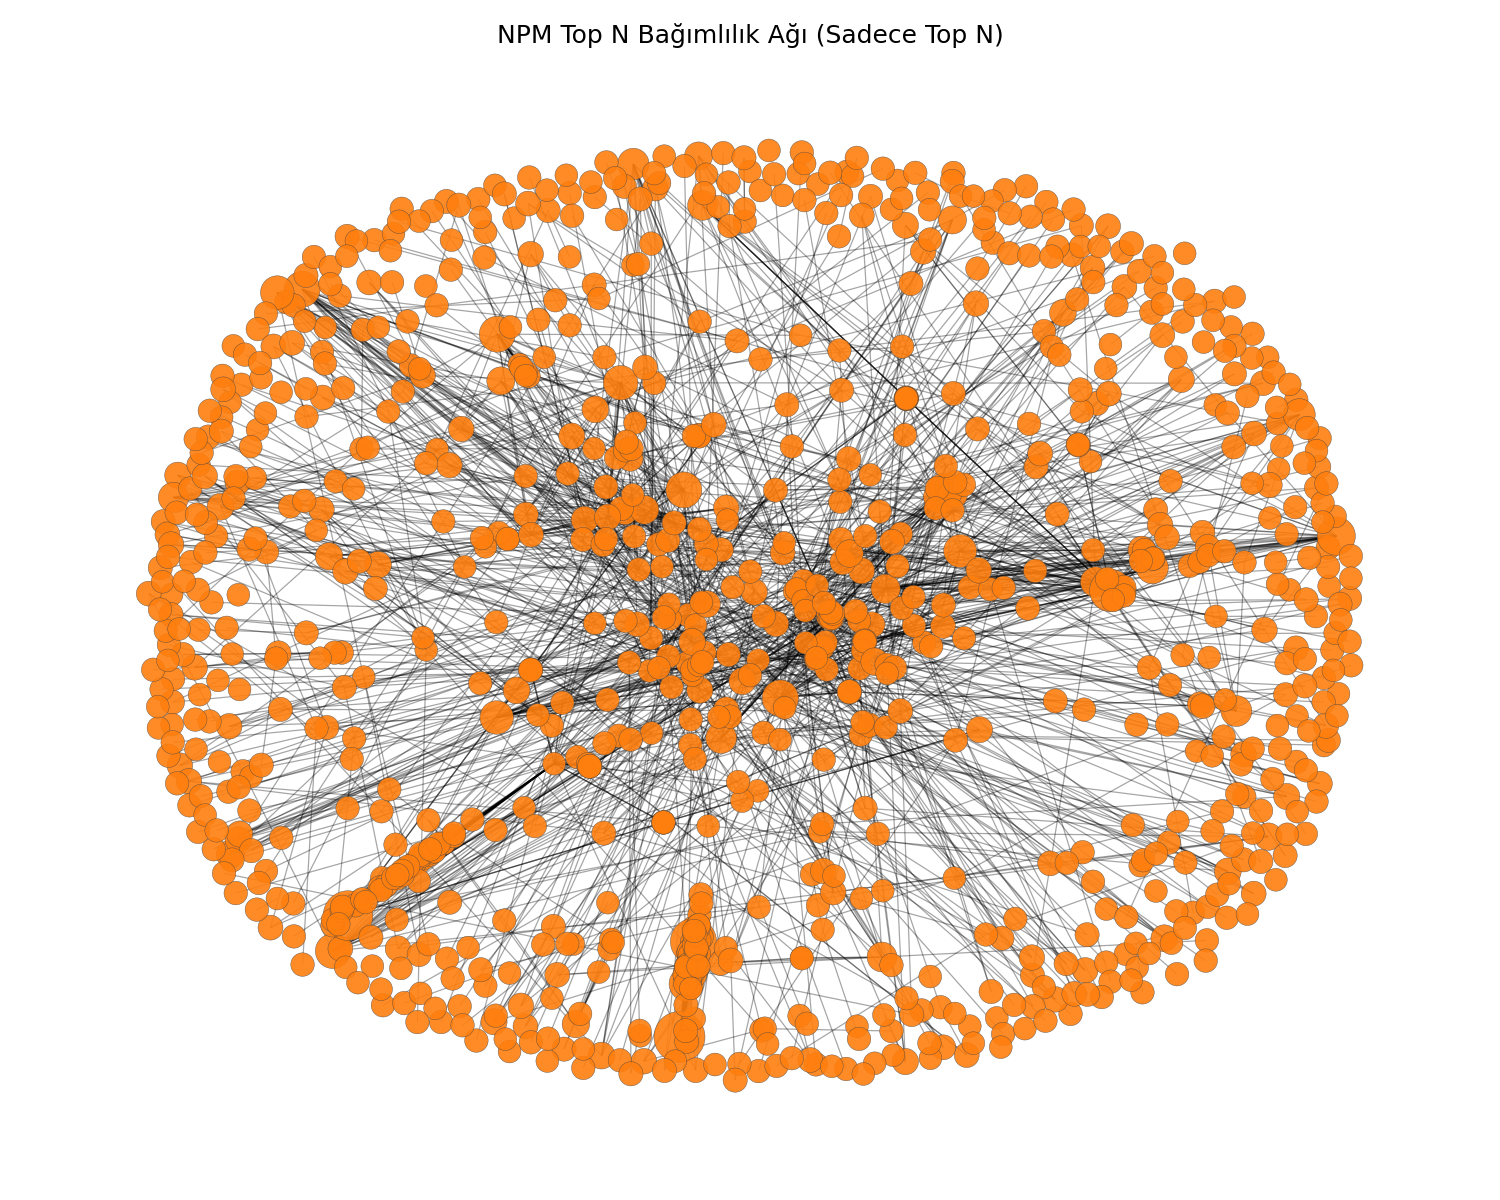
\includegraphics{network_topN_only.png}
  \caption{Sadece Top~N düğümlerin indüklenmiş alt-ağı. Paketin ağ içi konumuna göre merkezî (yüksek in-degree/betweenness) düğümler görselde öne çıkar.}
\end{figure}

\noindent Top~N alt-ağında bağlantı motifleri daha belirgindir. Zincirleme etkinin Top~N içinde nasıl yayılabileceğini niteliksel olarak gözlemlemek mümkündür.

\subsection{Derece Dağılımları ve İlişkiler}
\begin{figure}[H]
  \centering
  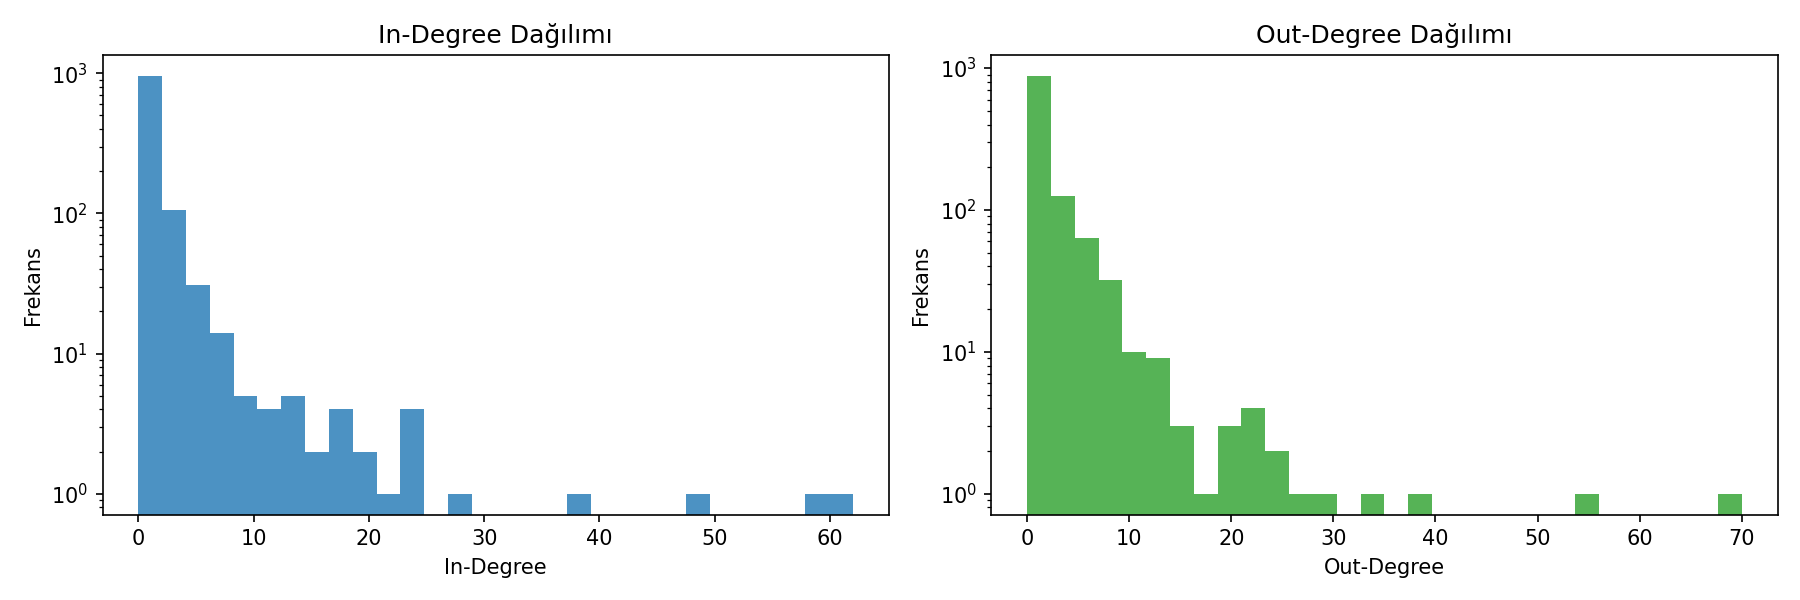
\includegraphics{degree_histograms.png}
  \caption{In-degree ve out-degree histogramları (log ölçek). Ağın kuyruklarının ağır olması, az sayıda çok etkili paket ile çok sayıda düşük dereceye sahip paketin birlikte varlığını gösterir.}
\end{figure}

\noindent In-degree dağılımı, sistemik etkisi yüksek omurga paketleri az sayıda düğümde toplar. Out-degree dağılımı, bazı paketlerin geniş bağımlılık yüzeyi nedeniyle tedarik riskine daha açık olduğunu gösterir.

\begin{figure}[H]
  \centering
  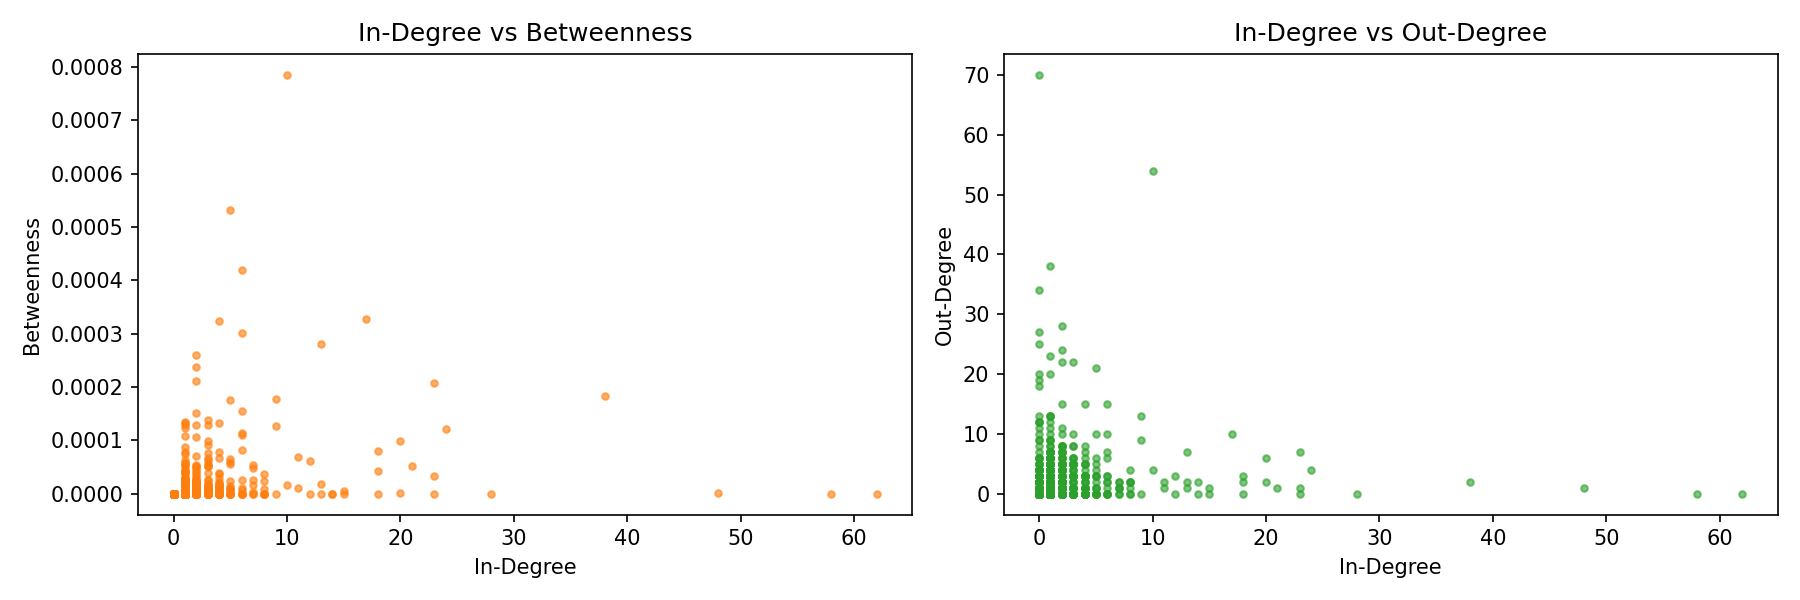
\includegraphics{scatter_correlations.png}
  \caption{Korelasyonlar: (sol) In-degree vs Betweenness; (sağ) In-degree vs Out-degree. In-degree ile betweenness arasındaki pozitif ilişki, omurga düğümlerin çoğu zaman köprü rolünde olduğunu gösterir.}
\end{figure}

\noindent In-degree ile out-degree ilişkisi, bir paketin hem çok kullanılıyor hem de çok sayıda bağımlılığa sahip olabildiğini; bu durumda hem yayılım hem maruziyet riskinin birlikte arttığını gösterir.

\subsection{Merkeziyet Liderleri}
\begin{figure}[H]
  \centering
  \begin{subfigure}[t]{0.48\textwidth}
    \centering
    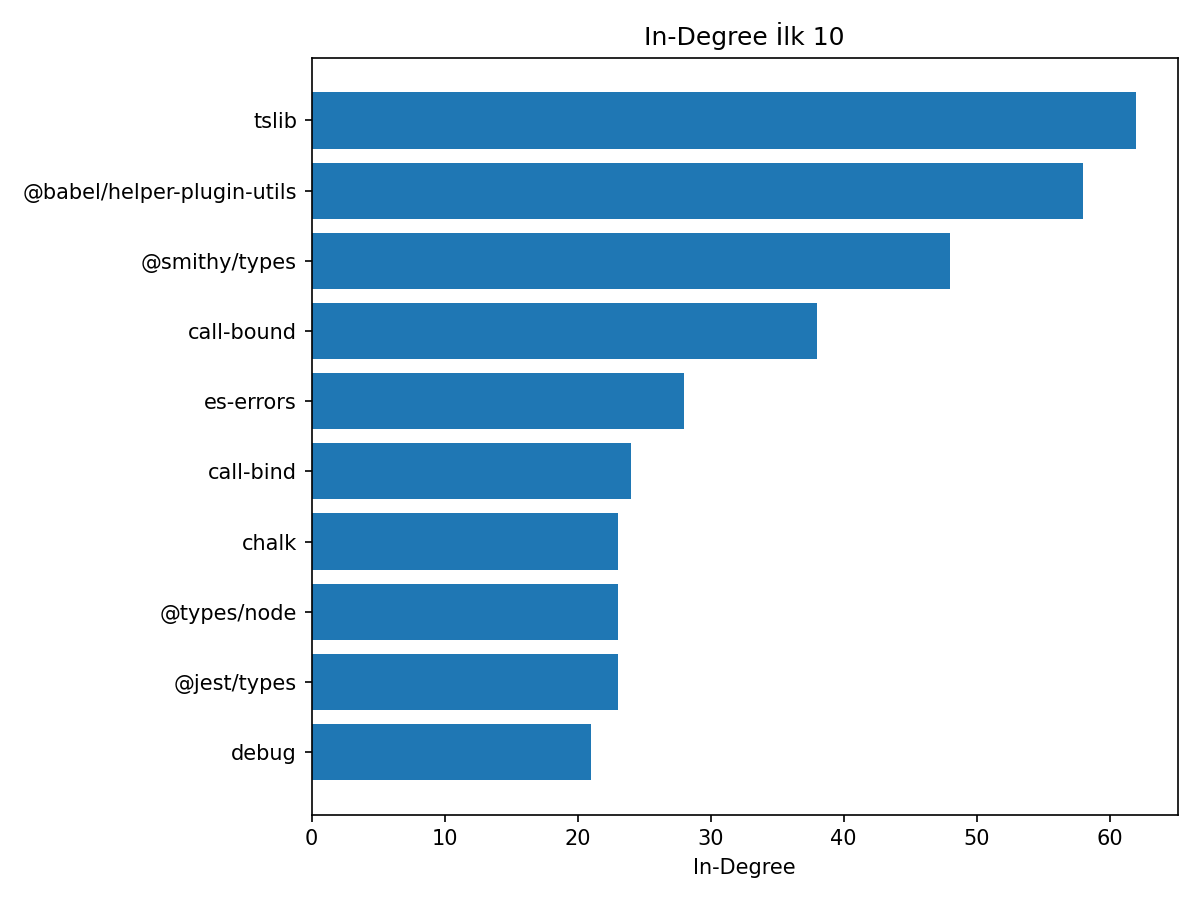
\includegraphics{top10_in_degree.png}
    \caption{İlk 10 In-degree}
  \end{subfigure}\hfill
  \begin{subfigure}[t]{0.48\textwidth}
    \centering
    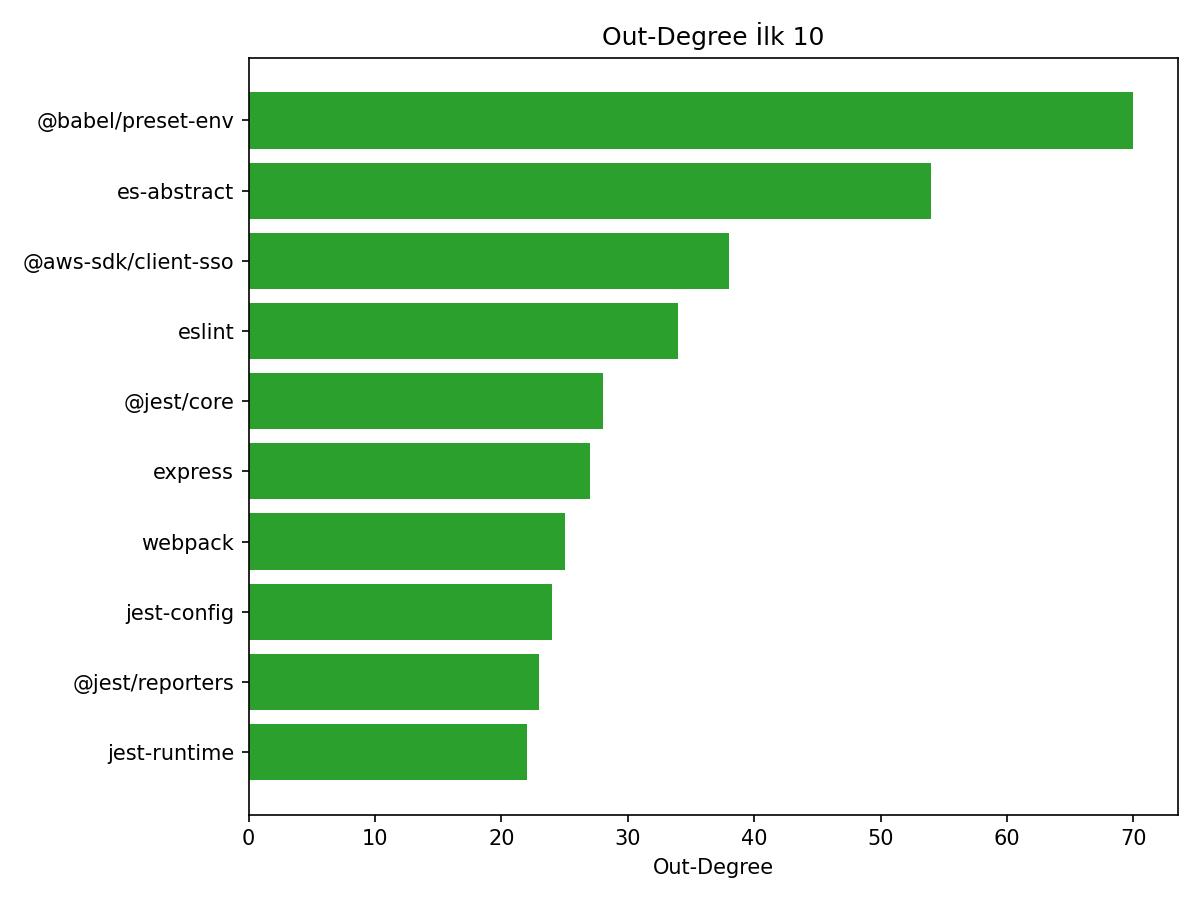
\includegraphics{top10_out_degree.png}
    \caption{İlk 10 Out-degree}
  \end{subfigure}
  \caption{Derece liderleri. In-degree liderleri yayılım etkisi yüksek paketlerdir; out-degree liderleri ise bağımlılık yüzeyi geniş paketlerdir.}
\end{figure}

\noindent In-degree listesi, transitif etki alanı geniş paketleri işaret eder. Out-degree listesi, tedarik yüzeyi geniş olduğu için arıza/bozulmalara duyarlılığı artan paketleri vurgular.

\begin{figure}[H]
  \centering
  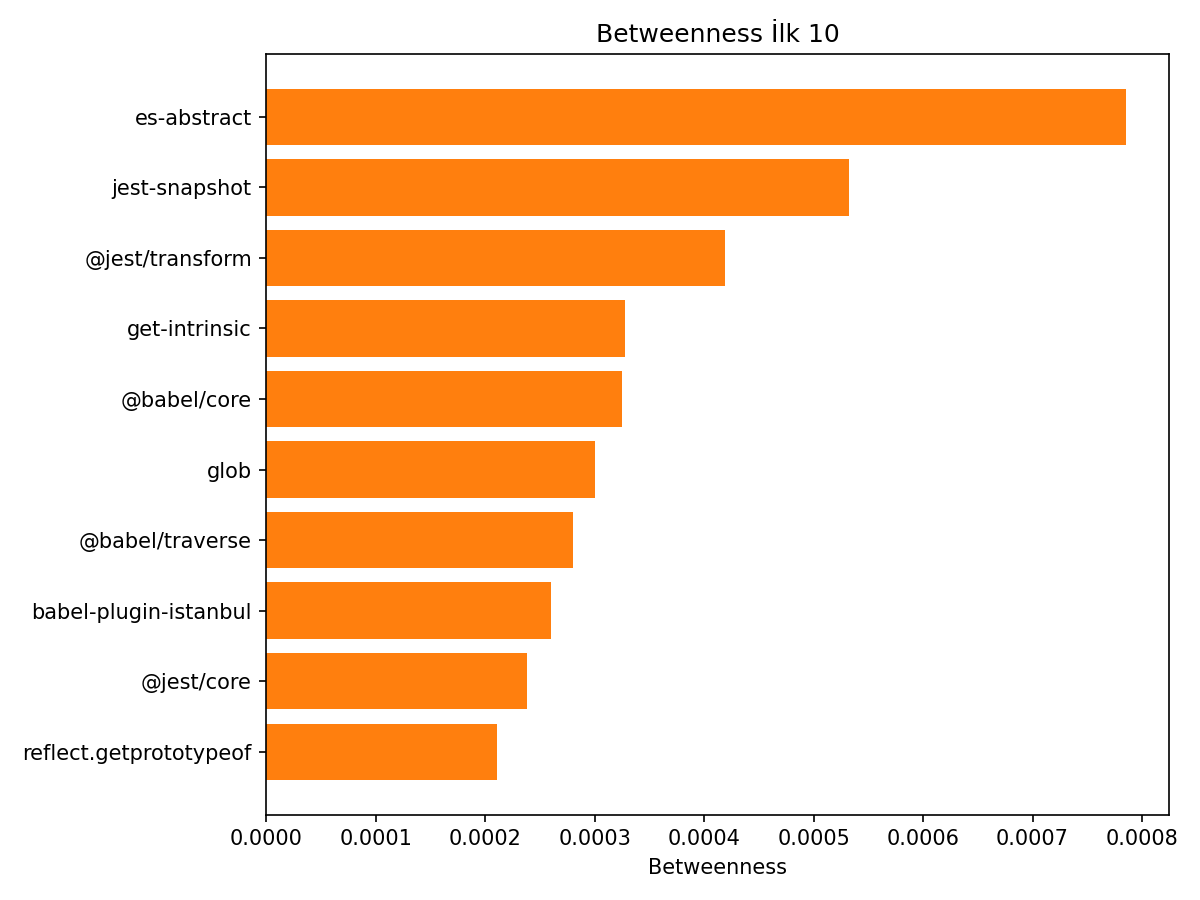
\includegraphics{top10_betweenness.png}
  \caption{İlk 10 Betweenness. Bu düğümler en kısa yollarda köprü rolündedir; tek hata noktası riski taşırlar.}
\end{figure}

\noindent Yüksek betweenness, topolojideki alt-ağlar arası akışın bir düğümde yoğunlaştığını ve bu düğümün potansiyel bir boğaz noktası olduğunu gösterir.

\subsection{Bileşik Risk Skoru}
\begin{figure}[H]
  \centering
  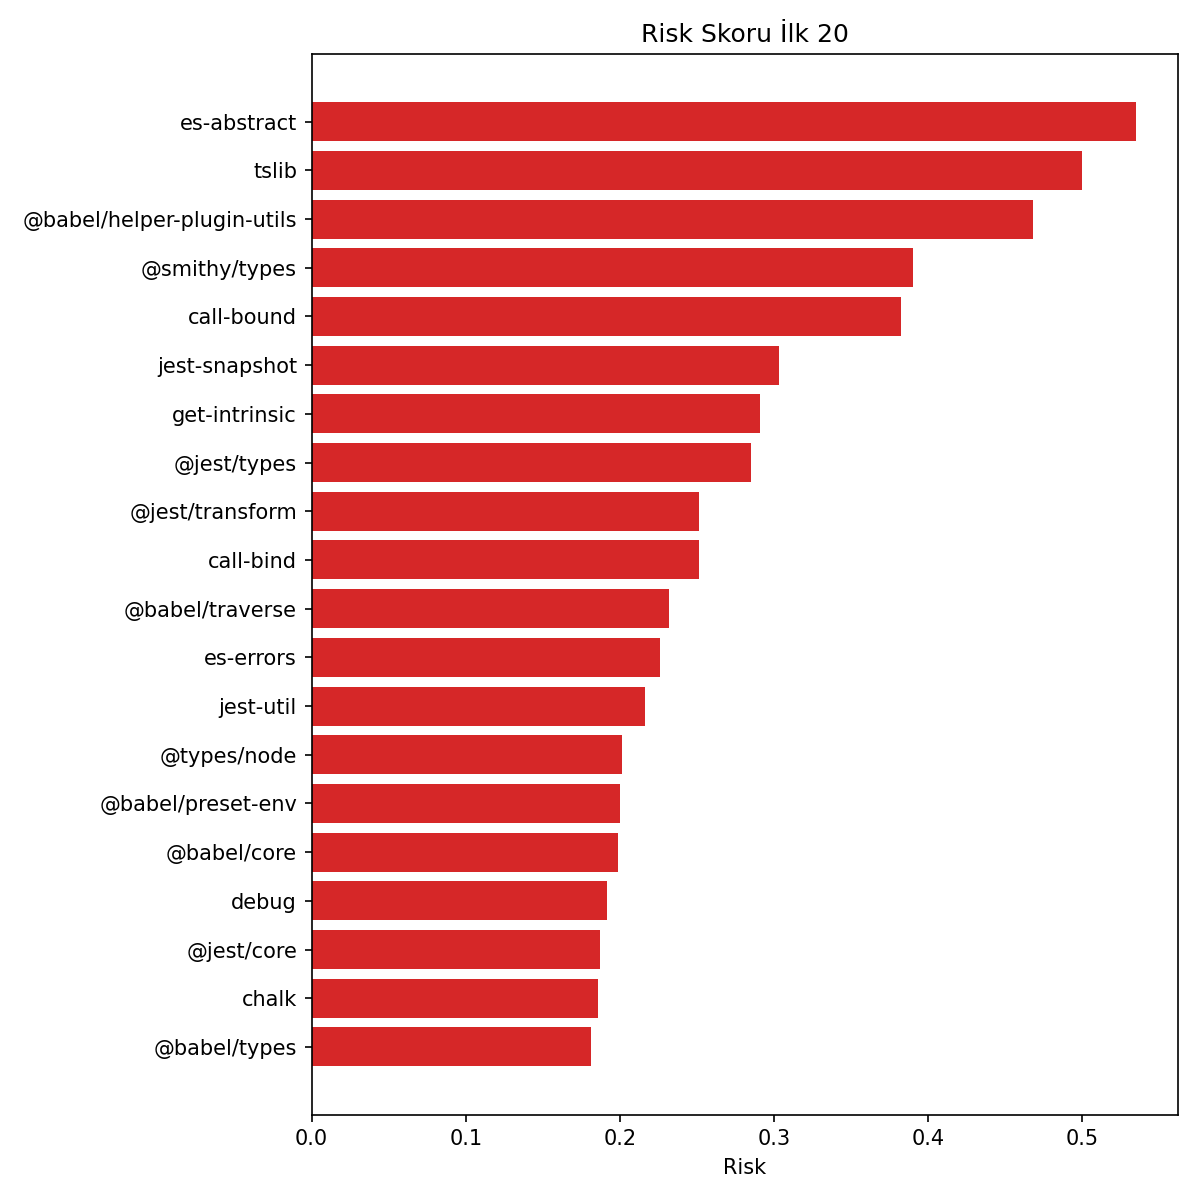
\includegraphics{top20_risk.png}
  \caption{Bileşik risk skoru ile en riskli 20 paket. Ağırlıklar in/out/betweenness arasında denge kuracak biçimde seçilmiştir.}
\end{figure}
\IfFileExists{../results/risk_scores_top20.tex}{\begin{longtable}{lrrrrr}
\caption{Top 20 Risk Skoru}\\
\toprule
Paket & Risk & In-Degree & Out-Degree & Betweenness & TopN? \\
\midrule
\endfirsthead
\toprule
Paket & Risk & In-Degree & Out-Degree & Betweenness & TopN? \\
\midrule
\endhead
\bottomrule
\endfoot
\bottomrule
\endlastfoot
es-abstract & 0.534931 & 10 & 54 & 0.000785 & True \\
tslib & 0.500000 & 62 & 0 & 0.000000 & True \\
@babel/helper-plugin-utils & 0.467742 & 58 & 0 & 0.000000 & True \\
@smithy/types & 0.390249 & 48 & 1 & 0.000001 & True \\
call-bound & 0.382129 & 38 & 2 & 0.000183 & True \\
jest-snapshot & 0.303511 & 5 & 21 & 0.000532 & True \\
get-intrinsic & 0.290993 & 17 & 10 & 0.000328 & True \\
@jest/types & 0.284735 & 23 & 7 & 0.000207 & True \\
@jest/transform & 0.251456 & 6 & 15 & 0.000419 & True \\
call-bind & 0.251171 & 24 & 4 & 0.000121 & True \\
@babel/traverse & 0.231984 & 13 & 7 & 0.000280 & True \\
es-errors & 0.225806 & 28 & 0 & 0.000000 & True \\
jest-util & 0.216164 & 20 & 6 & 0.000099 & True \\
@types/node & 0.201331 & 23 & 1 & 0.000034 & True \\
@babel/preset-env & 0.200000 & 0 & 70 & 0.000000 & True \\
@babel/core & 0.199075 & 4 & 15 & 0.000324 & True \\
debug & 0.191845 & 21 & 1 & 0.000051 & True \\
@jest/core & 0.187008 & 2 & 28 & 0.000238 & True \\
chalk & 0.185484 & 23 & 0 & 0.000000 & True \\
@babel/types & 0.181088 & 18 & 2 & 0.000079 & True \\
\end{longtable}
}{\fbox{risk\_scores\_top20.tex bulunamadı}}

\noindent Tablo sütunları: Risk (0--1 aralığında normalize), In-Degree (pakete bağımlı paket sayısı), Out-Degree (paketin bağımlılık sayısı), Betweenness (en kısa yollardaki köprü rolü), TopN? (Top~N listesinde olup olmadığı). Liste, derleme/test altyapısında yer alan ve geniş yayılıma sahip kütüphanelerin (ör. Babel/Jest/TypeScript ekosistemleri) sistemik risk potansiyeline işaret eder.

\subsection{Kaskad Etkisi ve Sağlamlık}
\begin{figure}[H]
  \centering
  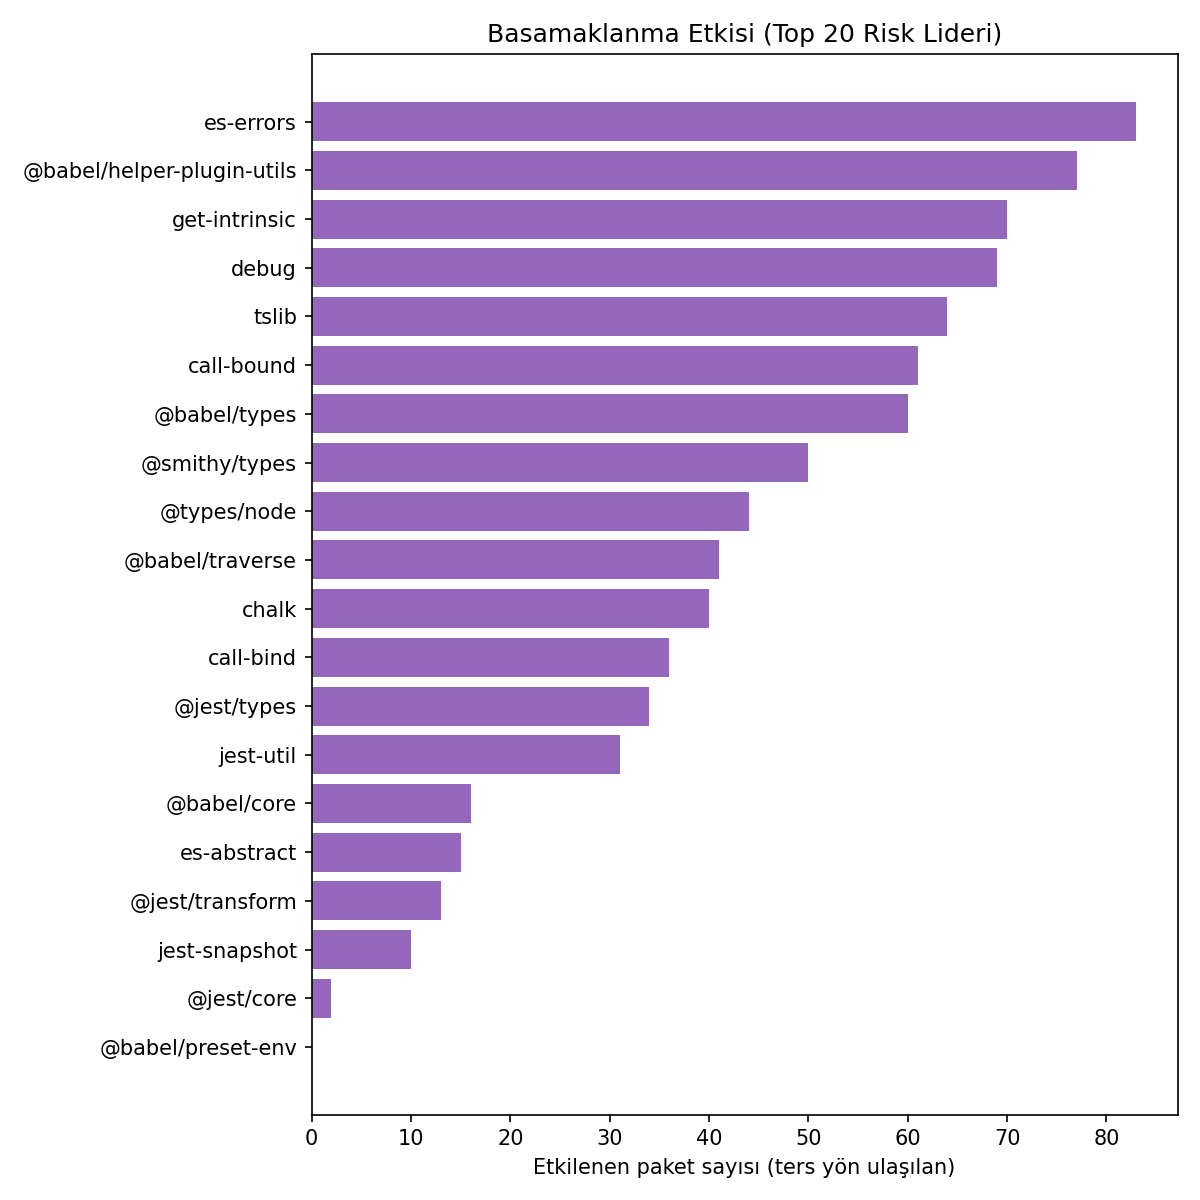
\includegraphics{cascade_impact_top20.png}
  \caption{Risk skoruna göre en riskli 20 paket için kaskad etki büyüklüğü. Yüksek risk genellikle daha büyük kaskada karşılık gelse de, topolojiye bağlı istisnalar görülebilir.}
\end{figure}
\IfFileExists{../results/cascade_impact_top20.tex}{\begin{table}[h]
\centering
\caption{Basamaklanma Etkisi: Top 20 (Ters y"onde etkilenebilecek paket say\i s\i)}
\begin{tabular}{l r}
\toprule
Paket & Etkilenen Paket Say\i s\i \\ \midrule
es-errors & 83 \
@babel/helper-plugin-utils & 77 \
get-intrinsic & 70 \
debug & 69 \
tslib & 64 \
call-bound & 61 \
@babel/types & 60 \
@smithy/types & 50 \
@types/node & 44 \
@babel/traverse & 41 \
chalk & 40 \
call-bind & 36 \
@jest/types & 34 \
jest-util & 31 \
@babel/core & 16 \
es-abstract & 15 \
@jest/transform & 13 \
jest-snapshot & 10 \
@jest/core & 2 \
@babel/preset-env & 0 \
\bottomrule
\end{tabular}
\end{table}
}{\fbox{cascade\_impact\_top20.tex bulunamadı}}

\begin{figure}[H]
  \centering
  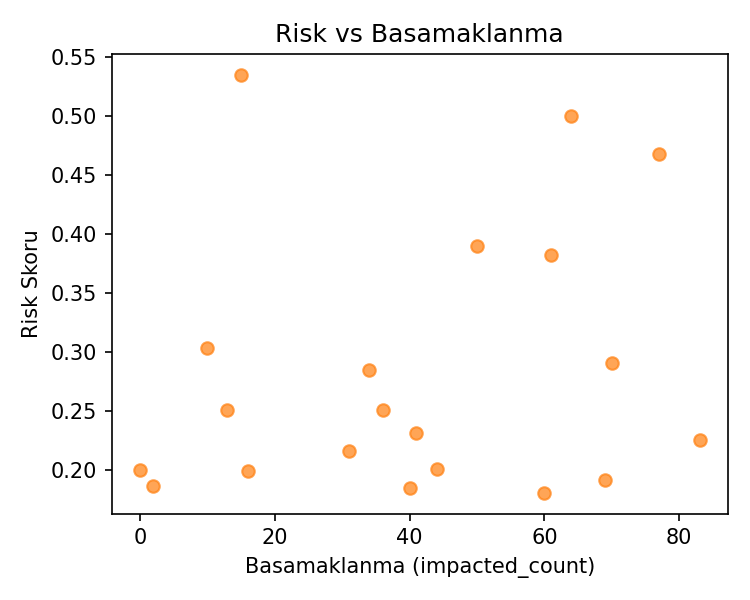
\includegraphics{risk_vs_cascade.png}
  \caption{Risk skoru ile kaskad etkisi ilişkisi (scatter). Doğrusal olmayan yapı, tek başına derece metriklerinin tüm yayılım dinamiğini açıklamadığını gösterir.}
\end{figure}

\noindent Kaskad etkisi, ağın bağlantı yapısına duyarlıdır: Aynı risk puanına sahip iki düğüm, komşuluklarının farklılığı nedeniyle farklı kaskad profilinde sonuçlar doğurabilir.

\subsection{Köprü Kenarlar}
\noindent En yüksek edge betweenness değerine sahip kenarlar, alt-ağlar arasında kırılgan bağlantıları işaret eder; bu kenarlar üzerindeki trafik, topolojik ayrışma noktalarını anlamaya yardımcı olur.
\IfFileExists{../results/edge_betweenness_top10.tex}{\begin{longtable}{l l r}
\caption{Edge Betweenness Ilk 10 (Yuksek kopru kenarlar)}\\
\toprule
U & V & Edge Betweenness \\
\midrule
\endfirsthead
\toprule
U & V & Edge Betweenness \\
\midrule
\endhead
\bottomrule
\endfoot
\bottomrule
\endlastfoot
@jest/transform & babel-plugin-istanbul & 0.000222 \\
@jest/expect & jest-snapshot & 0.000212 \\
jest-snapshot & @jest/transform & 0.000206 \\
jest & @jest/core & 0.000150 \\
call-bound & get-intrinsic & 0.000150 \\
glob & jackspeak & 0.000147 \\
reflect.getprototypeof & which-builtin-type & 0.000146 \\
jackspeak & @isaacs/cliui & 0.000140 \\
babel-plugin-istanbul & test-exclude & 0.000139 \\
@babel/core & @babel/helper-compilation-targets & 0.000138 \\
\end{longtable}
}{\fbox{edge\_betweenness\_top10.tex bulunamadı}}

\subsection{Ağın Temel İstatistikleri}
\IfFileExists{../results/graph_stats.tex}{\begin{longtable}{l r}
\caption{Graf İstatistikleri (özet)}\\
\toprule
Ölçüt & Değer \\
\midrule
\endfirsthead
\toprule
Ölçüt & Değer \\
\midrule
\endhead
\bottomrule
\endfoot
\bottomrule
\endlastfoot
\textbf{Düğüm sayısı} & 1139 \\
\textbf{Kenar sayısı} & 2164 \\
\textbf{Bileşen sayısı (zayıf)} & 160 \\
\textbf{En büyük bileşen boyutu} & 853 \\
Ortalama in-degree & 1.8999 \\
Ortalama out-degree & 1.8999 \\
\end{longtable}

}{\fbox{graph\_stats.tex bulunamadı}}

\noindent Bu özet tabloda düğüm/kenar sayıları, zayıf bağlanırlık bileşen sayısı, en büyük bileşen boyutu ve ortalama dereceler raporlanır. Zayıf (weak) bileşen, kenar yönleri yok sayıldığında bağlı olan düğüm kümeleridir.

\section{Sınırlamalar}
\textbf{Kapsam.} Varsayılan olarak yalnızca dependencies alanı kullanılmıştır; peerDependencies isteğe bağlıdır. Global dependent sayıları doğrudan dahil edilmemiştir.

\textbf{Betweenness.} Büyük graflarda betweenness için örnekleme zorunludur; yakınsama, ağ büyüklüğü ve $k$ seçimine bağlıdır.

\section{Sonuç}
NPM ekosistemi, az sayıda omurga ve köprü paket etrafında yoğunlaşan bir topoloji sergiler. Bileşik risk skoru ve sağlamlık bulguları, tedarik zinciri güvenliğinde yapısal bakışın analitik değerini açıkça ortaya koyar.

\paragraph{Tekrarlanabilirlik.} Tüm kod ve çıktı üretimi depo içindedir. analysis.ipynb çalıştırılarak results/ çıktıları yeniden üretilebilir ve bu makale derlenebilir.

\end{document}
